\documentclass[12pt]{scrreprt}
\usepackage{fontspec,microtype}
\usepackage[ngerman]{babel}
\usepackage[utf8]{inputenc}
\usepackage[T1]{fontenc}
\usepackage{ae}
\usepackage{graphicx}
\usepackage{hyperref}
%\usepackage[printonlyused,withpage]{acronym}
\usepackage[acronym,toc,section]{glossaries}
\usepackage{subfig}
\usepackage{setspace}

\usepackage{geometry}
\geometry{a4paper, top=15mm, left=35mm, right=25mm, bottom=15mm}

%Fancy Kapitelübersxchrift und Textfont
\usepackage{lmodern,titlesec,tikz,blindtext}
\newcommand*{\chapnumfont}{\normalfont\huge\bfseries}
\titleformat{\chapter}[display]
{\filleft\bfseries}
{\filleft%
  \begin{tikzpicture}
    \draw[fill,color=black] (0,0) rectangle (2cm,2cm);
    \draw[color=white] (1cm,1cm) node {\chapnumfont\thechapter};
  \end{tikzpicture}
}
{20pt}
{\Huge}
\setmainfont{Minion Pro}
\setsansfont{Myriad Pro}

\newglossary[slg]{symbolslist}{syi}{syg}{Symbolverzeichnis}
\renewcommand*{\glspostdescription}{}
\makenoidxglossaries
%Befehle für Symbole
\newglossaryentry{symb:Pi}{
name=$\pi$,
description={Die Kreiszahl.},
sort=symbolpi, type=symbolslist
}


%Befehle für Abkürzungen
\newacronym{acr:AR}{AR}{Augmented Reality}
\newacronym{acr:VR}{VR}{Virtual Reality}
\newacronym{acr:UE}{UE}{Unity Engine}
\newacronym{acr:UE4}{UE4}{Unreal Engine 4}
\newacronym[plural={\glspl{glos:SDK}}]{acr:SDK}{SDK}{\gls{glos:SDK}}
\newacronym{acr:knn}{KNN}{Künstliche Neuronale Netze}
\newacronym{acr:UI}{UI}{User Interface}
\newacronym{acr:IDS}{IDS}{Interne Datenstruktur}


\newglossaryentry{glos:SDK}{%
  name={Software Development Kit},
  description={TODO},
  plural={Software Development Kits}
}

\newglossaryentry{glos:Workflow}{%
  name={Workflow},
  description={TODO},
}

\newglossaryentry{glos:OpenSrc}{%
  name={Open Source},
  description={TODO},
}

\newglossaryentry{glos:Labeling}{%
  name={Labeling/Datennotation/Klassifizierung},
  description={TODO},
  plural={Labeln}
}

\newglossaryentry{glos:Tiefenkamera}{%
  name={Tiefenkamera},
  description={TODO},
  plural={Tiefenkameras}
}

\newglossaryentry{glos:Umfeldmodell}{%
  name={Tiefenkamera},
  description={TODO},
  plural={Umfeldmodelle}
}

\newglossaryentry{glos:Roomscaling}{%
  name={Roomscaling},
  description={TODO}
}

\newglossaryentry{glos:Debugger}{%
  name={Debugging-Tool},
  description={TODO},
  plural={Debugging-Tools}
}

\newglossaryentry{glos:Taktrate}{%
  name={Taktrate},
  description={TODO}
}

\newglossaryentry{glos:UI}{%
  name={User Interface},
  description={TODO},
  plural={User Interfaces}
}

\newglossaryentry{glos:Scripting}{%
  name={Scripting},
  description={TODO}
}

\newglossaryentry{glos:PostPr}{%
  name={Post Processing},
  description={TODO}
}

\newglossaryentry{glos:Shader}{%
  name={Shader},
  description={TODO}
}

\newglossaryentry{glos:GameEngine}{%
  name={Game Engine},
  description={TODO}
}

\newglossaryentry{glos:PredAna}{%
  name={Predictive Analytics},
  description={TODO}
}

\makeindex


\begin{document}
\onehalfspacing
%\sffamily


\title{
	{Entwicklung einer VR-basierten Methode für 3D-Datennotation}\\
	{\large Cmore Automotive GmbH}\\
	{
\includegraphics{Main_Images/cmoreLogo}}
}
\author{Patrick Grüner}
\date{\today}
\maketitle

\pagenumbering{roman}
\tableofcontents

\newpage
\chapter*{Abstract}
Abstract goes here

\chapter*{Dedication}
To mum and dad

\chapter*{Declaration}
I declare that..

\chapter*{Acknowledgements}
I want to thank...
\newpage

\newpage
\printnoidxglossary[style=altlist,title=Glossar]

\newpage
\deftranslation[to=German]{Acronyms}{Abkürzungsverzeichnis}
\printnoidxglossary[type=\acronymtype,style=long]

\newpage
\printnoidxglossary[type=symbolslist,style=long]

\newpage

\pagenumbering{arabic}
\chapter{Einleitung}
\graphicspath{{Kapitel/Kapitel1_Einleitung/Images/}}

Der Einsatz künstlicher Intelligenzen ist aktuell in allen Bereichen der Informatik auf dem Vormarsch. Dies gilt vor allem für die Automobilindustrie, da das Thema des autonomen Fahrens nicht ohne intelligente Algorithmen realisierbar ist. Eine wichtige Rolle bei der Entwicklung solcher Algorithmen spielt dabei das maschinelle Lernen. Dabei wird versucht, ausgehend von vielen lehrreichen Beispieldaten, die Lösung einer Aufgabe zu lernen und auf andere unbekannte Daten zu verallgemeinern. So kann ein System auch auf vorher ungesehene Daten reagieren, was mit einer statischen Programmierung nur schwer oder gar nicht möglich ist. Der Erfolg dieses Prinzips hängt genauso von der Qualität der Trainingsdaten ab wie der des Algorithmus. Deshalb wird in die Erstellung dieser Daten sehr viel Arbeit gesteckt.\\

Im Bereich der Fahrerassistenzsysteme und des autonomen Fahrens ist es wichtig, dass das Auto seine Umgebung so gut wie möglich wahrnehmen kann. Deshalb werden für Algorithmen, die in diesen Bereichen angewendet werden, Daten von Sensoren verwendet um das Umfeld des Autos wahrzunehmen. Dies sind meist Kamera-, Rader- oder Lidarsensoren. Die Eingangsdaten dieser Sensoren müssen nun so aufbereiten werden, damit ein lernendes Computersystem etwas damit anfangen kann. Dazu werden alle, für das Anwendungsfeld wichtigen Teile mit entsprechenden Klassifikationen versehen. Diese Klassifikationen werden auch als \textit{Labels} oder \textit{Annotationen} bezeichnet. Zum Beispiel werden auf einem Kamerabild alle Personen und Fahrzeuge als eben diese markiert. Das Fahrzeug kann auf diese Weise lernen wie Personen und Fahrzeuge aussehen, um sie dann später im Straßenverkehr selbstständig wiederzuerkennen. Radar- und Lidarsensoren liefern stattdessen Punktwolken als Eingangsdaten (vgl. Abbildung \ref{fig:Punktwolke}), das Prinzip bleibt allerdings das gleiche. Auch hier müssen alle wichtigen Teile, in diesem Fall Punkte, mit entsprechenden Klassen versehen werden. Dieser Vorgang nennt sich \textit{Labeln} bzw. \textit{Annotieren}.\\

\begin{figure}%
	\centering
    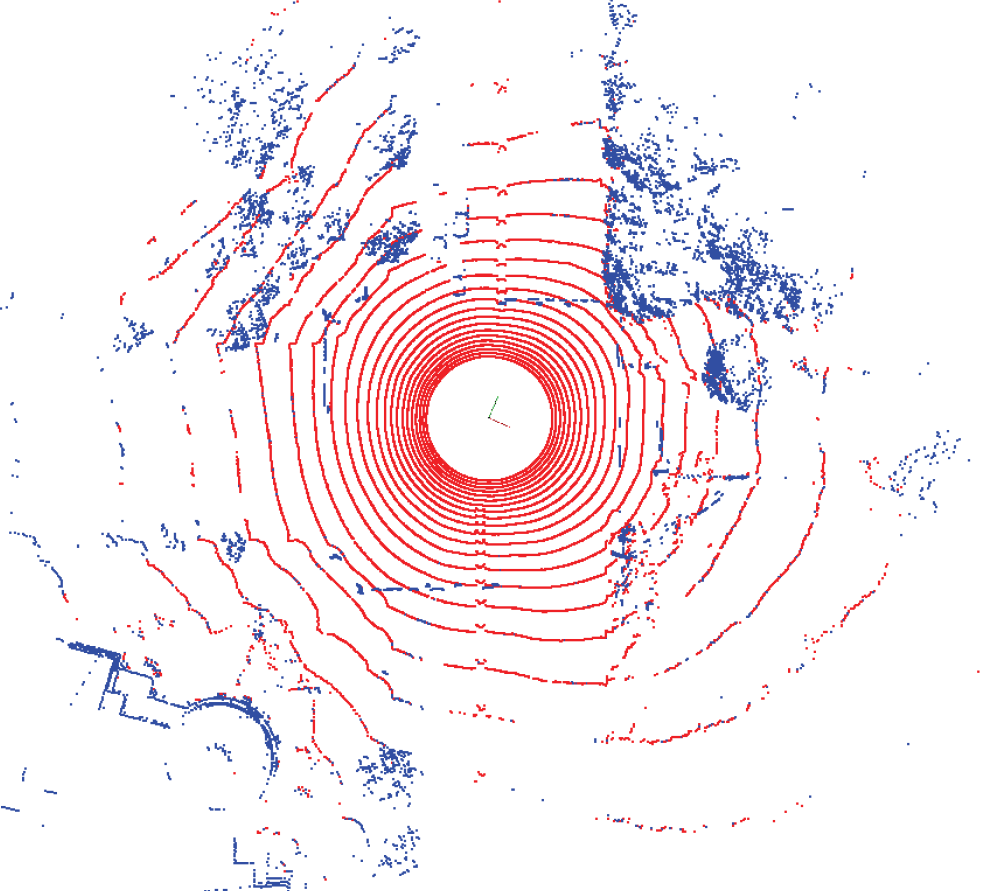
\includegraphics[width=7.5cm]{Punktwolke}
    \caption{Vogelperspektive auf eine Lidar-Punktwolke, wobei die roten Punkte alle Boden- und die blauen alle Nicht-Bodenpunkte darstellen \cite{bib:FastGroundSeg}}
	\label{fig:Punktwolke}
\end{figure}


\section{Motivation}
In einem bislang aufwändigen Verfahren (siehe Kapitel \ref{sec:C.LABEL}) müssen diese Punktwolken so aufbereitet und mit einer Bedeutung versehen werden, dass die Algorithmen an diesen Beispielen etwas lernen können. Sie müssen nach dem Lernen in der Lage sein Unterscheidungen und Erkennungen selbst durchzuführen und dabei möglichst wenige Fehler machen. Bei solchen Verfahren kommen Softwareanwendungen wie \textit{C.LABEL} zum Einsatz. Dies ist eine Anwendung zum Annotieren verschiedener Sensordaten für den Automobilbereich und wurde von der Firma \textit{CMORE Automotive GmbH} entwickelt. CMORE ist das betreuende Unternehmen dieser Masterarbeit und wird in Kapitel \ref{sec:CMORE} vorgestellt. Das Programm C.LABEL ist in Kapitel \ref{sec:C.LABEL} erklärt. C.LABEL ist eine Anwendung, die zunächst die Sensordaten für den menschlichen Benutzer visualisiert. Dieser muss sie dann manuell mit unterschiedlichen Bedeutungen versehen. Wegen der großen Menge an Daten, die für das Trainieren der Algorithmen benötigt wird, muss dieses manuelle Annotieren möglichst effizient durchführbar sein.\\

Ein zweidimensionales Kamerabild kann sehr einfach auf einem Computermonitor dargestellt und bearbeitet werden. Eine besondere Herausforderung stellt jedoch die Verarbeitung von 3D-Daten, wie einer Punktwolke, dar. Hier stößt man mit den Möglichkeiten eines zweidimensionalen Computermonitors schnell an die Grenzen einer effizienten Darstellung und Bearbeitung. So ist es beispielsweise für die Annotierung solcher Punktwolken und ihrer Einzelmesswerte schwierig, die optimale Perspektive auf die Daten zu finden, die eine effiziente Erfassung durch den Menschen und eine entsprechende Bearbeitung zulässt. Dies erfordert von den Benutzern sehr viel Übung und Erfahrung, durch entsprechende Drehungen der Punktwolkendarstellung sich in dieser zurechtzufinden und Messpunkte realen Objekten zuzuordnen.\\ 

Eine Alternative dazu soll diese Masterarbeit bieten, welche eine Applikation beschreibt, die das Visualisieren und Annotieren von Punktwolken einfacher und effizienter gestaltet. Mittels neuartiger Technologien wie Virtual- und Augmented Reality soll die Grenze zwischen 2-D und 3-D aufgehoben werden, sodass man sich als interaktiver Teilnehmer im dreidimensionalen Raum durch die Sensordaten navigieren, mit ihnen interagieren und sie annotieren kann.\\

\section{Ziel der Arbeit}
Ziel dieser Arbeit ist es zunächst ein passendes Medium für eine solche Applikation zu finden, das nicht nur die Anforderungen der Applikation selbst erfüllt, sondern auch an einem handelsüblichen Büro-Arbeitsplatz verwendet werden kann. Anschließend soll eine Applikation erstellt werden die folgende Grundfunktionalität erfüllt:\\

\begin{enumerate}
\item Mit der Anwendung soll es Möglich sein ein, bei CMORE gängiges, Datenformat einzulesen und alle nötigen Informationen daraus zu extrahieren

\item Aus den extrahierten Informationen soll eine Punktwolke generiert und innerhalb des gewählten Mediums visualisiert werden.

\item Der Benutzer muss die Möglichkeit haben durch die Punktwolke zu navigieren.

\item Die Applikation muss die Möglichkeit bieten jeden einzelnen Punkt mit einer Klassifikation versehen zu können. Dabei sollen Alleinstellungsmerkmale des gewählten Mediums benutzt werden, um eine vorzeigbare Verbesserung gegenüber der herkömmlichen Computer-Monitor-Annotation zu generieren. 

\item Alle getätigten Annotationen müssen in die eingelesenen Dateien zurückgeschrieben bzw. in neue Dateien exportiert werden.
\end{enumerate}

Anschließend sollen die Basisfunktionen erweitert und zusätzliche Funktionen hinzugefügt werden. Abhängig von der verbleibenden Zeit soll die Anwendung gemäß folgender Priorität erweitert werden:\\

\begin{enumerate}
\item Es sollen neue Möglichkeiten zur Annotation von Punkten implementiert werden.

\item Die Möglichkeit, eigene Klassifikationen für Punkte zu erstellen, soll hinzugefügt werden.

\item Neue Datenformate importieren.

\item Neue Navigationsmöglichkeiten implementieren.
\end{enumerate}

Am wichtigsten wäre hierbei also die Applikation um effiziente Möglichkeiten zum labeln von Punkten zu erweitern. Außerdem sollte es für den Benutzer möglich sein individuelle Klassifikationen anzulegen, um unterschiedliche Anwendungsgebiete abzudecken. Optional sind neue Navigationsmöglichkeiten und einlesbare Datenformate. 

\section{Umfeld der Arbeit}

\subsection{CMORE Automotive GmbH}
\label{sec:CMORE}

\subsection{C.LABEL}
\label{sec:C.LABEL}


\chapter{Vorbereitungen}
\graphicspath{{Kapitel/Kapitel2_Vorbereitungen/Images/}}

%TODO
Kurze Einleitung was alles vorbereitet wurde.

\section{Wahl des passenden Mediums} 
Um das \glslink{glos:Labeling}{Labeling} von Daten, insbesondere Punktwolken, im dreidimensionalem Raum zu verwirklichen, gibt es zwei wesentliche Technologien die dafür relevant erscheinen. Diese sind \acrfull{acr:AR} und \acrfull{acr:VR}.\\

Unter \acrlong{acr:AR} versteht man die direkte oder indirekte Sicht auf die reale, physische Welt, welche durch digitale Inhalte erweitert wird. Dies wird vor allem durch Smartphones oder \acrshort{acr:AR}-Brillen realisiert. Bei einem Smartphone hat man beispielsweise einen indirekten Blick auf die reelle Umgebung durch das Display, welches ein Live-Bild der Kamera anzeigt. Diesem Bild können nun digitale Inhalte hinzugefügt werden. Bei einer Brille (vgl. Abbildung \ref{fig:AR-Brillen}) sieht man durch die Gläser direkt auf die physische Welt. Hierbei fungieren die Gläser als Display, welche in der Lage sind holographische Objekte anzuzeigen. Dies führt zu einer, für den Benutzer, sehr immersiven Vermischung der realen und der digitalen Welt. Üblicherweise ist es bei diesen Brillen sogar möglich durch Gesten, die mittels Händen durchgeführt werden, mit den Hologrammen zu interagieren.\\

\acrlong{acr:VR} ist eine Technologie bei der spezielle \acrshort{acr:VR}-Brillen zum Einsatz kommen, welche keine Sicht mehr auf die reale Umgebung ermöglichen (vgl. Abbildung \ref{fig:VR-Brillen}). Das Blickfeld des Menschen wird hierbei komplett von einem Display abgedeckt, das sich im Inneren der Brille befindet. So kann dem Benutzer eine komplette virtuelle Welt angezeigt werden. Mittels kompatiblen Controllern (vgl. Abbildung \ref{fig:Oculus}) kann sich durch diese Welt bewegt bzw. mit ihr interagiert werden. Die Controller werden dabei von einem Sensor erfasst und somit können reale Bewegungen der Controller in die virtuelle Welt der Brille übersetzt werden.


\subsection{Eignung von \acrlong{acr:AR} und \acrlong{acr:VR} im Bezug auf 3D-Datennotation}
Im folgenden Abschnitt wird auf die positiven und negativen Aspekte der beiden Technologien eingegangen, um abzuwägen welche besser für \glslink{glos:Labeling}{3D-Labeling} geeignet ist.

\subsubsection{Eignung von \acrlong{acr:AR}}
Der, im Rahmen dieser Arbeit, entwickelte Prototyp zur \glslink{glos:Labeling}{3D-Datennotation} ist nicht nur als Nutzungssoftware geplant, sondern dient auch als Anschauungsmaterial, beispielsweise für Messen. Zieht man diese Tatsache in Betracht, eignet sich \acrlong{acr:AR} sehr gut für diesen Zweck. Es wirkt durch die Vermischung von realen und digitalen Inhalten nämlich sehr futuristisch. Zudem ist das direkte einblenden holographischer Inhalte, durch eine \acrshort{acr:AR}-Brille, zum Zeitpunkt der Erstellung dieser Arbeit, noch wenig verbreitet (Microsoft Hololens wurde nur wenige Tausend mal verkauft \cite{bib:HololensVerkaufszahlen}), was bei unwissenden Benutzern zu einem beeindruckenden Effekt führt. Des Weiteren bietet die \acrlong{acr:AR} Technologie viele, für zukünftige \glslink{glos:Labeling}{Labeling}-Methoden relevante, Möglichkeiten. Den heutigen \acrshort{acr:AR}-Brillen ist es durch \glspl{glos:Tiefenkamera} möglich Objekte und deren Distanzen zur Brille wahrzunehmen. Folglich könnte ein zukünftiger Ansatz sein, eine Punktwolke der Umgebung, wie sie in \ref{sec:C.LABEL} zu sehen ist, mit einer \acrshort{acr:AR}-Brille zu erstellen. Diese kann anschließend vor Ort, in der Umgebung in der die Punktwolke erstellt wurde, klassifiziert werden.\\ %TODO Dieser Ansatz könnte ausführlicher sein. 

Ein wichtiger Punkt der ebenfalls betrachtet werden muss ist die Bedienung der Brille bzw. die Interaktion mit den digital dargestellten Objekten und Informationen. Die Steuerung von \acrshort{acr:AR}-Brillen erfolgt handelsüblich über Gesten, welche mit der Hand bzw. den Händen getätigt werden. Ob diese Art der Interaktion für den hier gewünschten Anwendungsfall passend wäre, lässt sich im Voraus schwer feststellen. Denkbar wäre, dass sich der Benutzer durch intuitive Gesten, die man auch bei realen Objekten nutzt, schnell an die Bedienung des Tools gewöhnen würde. Andererseits könnte die Selektion der Elemente einer Punktwolke zu ungenau sein, da die Brille die Position der Hand nicht richtig interpretiert bzw. diese nicht richtig zur Position der digitalen Inhalte interpretiert. Eine genaue Einschätzung der Bedienung für solch einen Anwendungsfall kann allerdings nur gegeben werden indem man einen \glslink{glos:Labeling}{Labeling}-Prototypen erstellt und ihn anschließend über längere Zeit testet. Dies ist im Zeitrahmen einer Masterarbeit jedoch nicht möglich. Falls sich nämlich die Steuerung als ungeeignet herausstellt bleibt nicht genug Zeit für eine Neuentwicklung auf einer anderen Plattform.\\  

Darüber hinaus gibt es natürlich auch Aspekte die gegen die \acrshort{acr:AR}-Technologie sprechen. Die \glslink{glos:Labeling}{Klassifizierung} einer Punktwolke mit dieser Technik ist an einem normalen Büro-Arbeitsplatz nicht möglich, zumindest nicht in einem Maßstab in dem es sinnvoll wäre. Die holographischen Punkte kollidieren, wenn sie darauf programmiert sind, mit der Umgebung und so würde Darstellung des \glslink{glos:Umfeldmodell}{Umfeldmodells} verfälscht werden. Auch wenn sie das nicht tun, dann wäre die Umgebung selbst immer noch ein Hindernis für den Benutzer, denn man möchte sich ja durch die Punktwolke bewegen. Des Weiteren sind bei \acrshort{acr:AR}-Brillen die vorherrschenden Lichtbedingungen ein großer Faktor, welche die Funktionalität gewisser Anwendungsfälle beeinflussen können. Wird beispielsweise eine Lichtquelle zu sehr von einem Objekt reflektiert, kann dieses von der \gls{glos:Tiefenkamera} der Brille nicht mehr richtig erfasst werden. Somit stimmt das \gls{glos:Umfeldmodell} nicht mehr mit der Realität überein. Zudem wird nicht nur die Funktionalität von Lichteinflüssen gestört, sondern auch die Darstellung der Hologramme. Bei zu viel Licht sind diese deutlich schwerer zu erkennen, vergleichbar mit der Nutzung eines Laptops im Freien, bei dem der Bildschirminhalt wegen zu heller Umgebung ebenfalls schlecht erkennbar ist. Für die Entwicklung selbst ist es ebenfalls hinderlich das es, zum Zeitpunkt der Erstellung dieser Arbeit, wenig Dokumentationen und Hilfestellungen, zum Beispiel in Entwicklerforen, gibt. Dies ist jedoch üblich für Technologien, die noch nicht lange auf dem Markt sind. Zu guter Letzt ist noch der finanzielle Faktor zu berücksichtigen. Durch die Aktualität der Technologie ist diese auch sehr teuer. Der Preis für eine \acrshort{acr:AR}-Brille kann dabei den Betrag von 5.000 Euro überschreiten, wie im  Abschnitt \ref{sec:ARVergleich} näher erläutert wird.    

\subsubsection{Eignung von \acrlong{acr:VR}} 

Die \acrlong{acr:VR} Technologie bietet den großen Vorteil, beliebig große Räume virtuell begehbar zu machen, ohne sich in der realen Welt selbst bewegen zu müssen. Dies ermöglicht die Bewegung durch Punktwolken, die im dreidimensionalen Raum dargestellt sind, an jedem üblichen Arbeitsplatz eines Büros. Des weiteren wirkt die Steuerung der \acrshort{acr:VR}-Brillen mittels den zugehörigen Controllern zum teil sehr ausgereift. Die Positions- und Bewegungserkennung des Benutzers wird als \textit{\glqq äußerst präzise\grqq} beschrieben \cite{bib:ControllerTest}. Dies ist sehr wichtig um die Handhabung der Anwendung für den späteren Endnutzer so angenehm wie möglich zu machen. Für die Entwicklung von \acrshort{acr:VR}-Applikationen selbst ist zu sagen, dass es mittlerweile sehr Umfassende Dokumentationen, Anleitungen und Beiträge zu den jeweiligen Plattformen und \glspl{acr:SDK} gibt. Dies hängt damit zusammen, dass sich die \acrlong{acr:VR} Technologie schon etwas länger auf dem Markt befindet und die Zahl der Entwickler für \acrshort{acr:VR}-Applikationen stetig steigt. Dies ist vermutlich nicht zuletzt der Tatsache zu verdanken, dass die Preise für \acrshort{acr:VR}-Brillen gesunken sind. Wie im späteren, ausführlicher beschreibenden, Abschnitt \ref{sec:ARVergleich} gezeigt, beträgt der aktuelle Preis einer Oculus Rift 449 Euro. Sowohl die zahlreichen Informationen für Entwickler als auch der niedrige Preis der Hardware sprechen, neben den zuvor genannten Aspekten, für die Wahl von \acrlong{acr:VR} als Plattform für die Entwicklung von 3D-\glslink{glos:Labeling}{Labeling}.\\

Was mit der \acrshort{acr:VR}-Technologie nicht ohne Weiteres funktioniert, ist die physische Begehung einer, zu \glslink{glos:Labeling}{klassifizierenden}, Punktwolke. Zwar bietet die Technik die Möglichkeit durch zusätzliche Sensoren die Bewegungen des Benutzers in die virtuelle Welt zu übersetzen, jedoch funktioniert dies nur auf begrenztem Raum und ist unmöglich an einem üblichen Büro-Arbeitsplatz durchführbar. Der reale begehbare Raum muss nämlich durch diese Sensoren abgesteckt werden und ist somit durch deren Reichweite und Genauigkeit begrenzt. Ein weiter Negativaspekt ist, dass viele Benutzer von \acrshort{acr:VR}-Brillen über Übelkeit klagen. In manchen Tests sind es mehr als 50 Prozent aller Teilnehmer, vor allem wenn es sich um Frauen handelt \cite{bib:VRSickness}. 


\subsection{\acrshort{acr:AR}-Brillen im Vergleich}
\label{sec:ARVergleich}
Zum Zeitpunkt der Recherche über eine passende \acrshort{acr:AR}-Brille, gibt es zwei potentielle Geräte die in Frage kommen. Diese sind Microsofts Hololens und die Meta 2. Andere Brillen werden, aufgrund der im voraus erkennbaren Hindernisse, nicht berücksichtigt, wie beispielsweise die Google Glass, die ein viel zu kleines Display hat. Wiederum andere sind zu diesem Zeitpunkt noch nicht auf dem Markt wie das Project Aurora, welches ebenfalls von Google ist, oder die Brille castAR. Im Folgenden werden die zwei potentiellen Brillen, im Hinblick auf die Nutzung für \glslink{glos:Labeling}{3D-Datennotation}, näher analysiert.

\subsubsection{Microsoft Hololens}
Die Hololens-Brille von Microsoft (vgl. Abbildung \ref{fig:Hololens}) punktet vorwiegend in Sachen Darstellung und räumlicher Interaktion, was aus eigener Erfahrung bekannt ist. Eingeblendete Hologramme wirken auf dieser Brille sehr stabil. Ein Ruckeln oder Nachpositionieren der digital dargestellten Inhalte wurde nie bemerkt. Ebenfalls gut funktioniert die Vermessung des Raums durch die Kameras der Brille. Hologramme interagieren dadurch sehr gut mit der physischen Umgebung, indem sie beispielsweise wie ein realer Gegenstand auf dem Tisch positioniert oder an die Wand gehängt werden können. Lediglich schlecht ausgeleuchtete Bereiche eines Raumes machen dieser Funktion Probleme, sodass die Brille beispielsweise eine Wand entdeckt wo gar keine ist. Die eben genannten Merkmale der Hololens, also eine stabile Darstellung und eine gute Einbettung einer Punktwolke in einen vorhandenen Raum, ist sehr wichtig um diese zuverlässig klassifizieren zu können und somit eine gute Methode für \glslink{glos:Labeling}{3D-Datennotation} zu entwickeln.\\
%evtl eigene Erfahrung noch reinbringen

Die Gestensteuerung der Hololens wäre für den Prozess der \glslink{glos:Labeling}{Klassifizierung} von dreidimensionalen Punktwolken eher ungeeignet. Durch Kopfbewegung müsste zum gewünschte Ziel navigiert und dieses dann mit einer Tipp-Geste in der Luft ausgewählt werden. Da dieser Vorgang schon beim Eingeben eines etwas komplexeren Passwortes Probleme bereitet, wäre er bei der Klassifikation von hunderten Punkten für den Benutzer sehr mühsam und langwierig. Ein weiter Punkt der negativ ins Gewicht fällt ist das kleine Sichtfeld der Brille. Tests sprechen hierbei von einer horizontalen Sichtweite die lediglich 30 bis 40 Grad beträgt \cite{bib:HololensTest}. Der Mensch kann dagegen horizontal fast 180 Grad wahrnehmen. Diese Eigenschaft würde den Benutzer daran hindern eine Punktwolke bzw. wenigstens einen Teilbereich dieser, als ganzes wahrzunehmen. Dadurch würde ein Großteil des Reizes verloren gehen, den die \glslink{glos:Labeling}{3D-Datennotation} bietet. Zudem ist die Hololens sehr teuer. Der Preis für die  Development Edition beträgt 3.299 Euro und in der Commercial Suite-Variante kostet die Brille sogar 5.489 Euro \cite{bib:HololensPreis}. Für eine prototypische Entwicklung die im Rahmen einer Abschlussarbeit angefertigt wird, ist das für ein Unternehmen ein sehr hoher Preis.

\subsubsection{Meta 2}
Für die Meta 2-Brille (vgl. Abbildung \ref{fig:Meta2}) spricht das hohe Sichtfeld, welches dem Hersteller nach 90 Grad beträgt und laut eines Tests \textit{\glqq hält, was es verspricht\grqq} \cite{bib:Meta2Test}. Wie im vorherigen Abschnitt angemerkt, ist ein hohes Sichtfeld sehr wichtig um dem Benutzer eine immersive Sicht auf eine Punktwolke zu geben. Die Steuerung der Brille wirkt ebenfalls gut und intuitiv. So ist es möglich Hologramme durch einfaches Greifen mit einer Hand auszuwählen, ohne diese zwangsläufig mit Kopfbewegungen anzuvisieren. Dies würde das selektieren vieler holographischer Gegenstände nacheinander erleichtern. Der Preis der Meta 2 ist, im Gegensatz zur Hololens geringer. Jedoch ist 1,495 Dollar immer noch ein hoher Betrag \cite{bib:Meta2Preis}.\\

Deutlich schlechter als die Hololens schneidet die Meta 2 bei der Performance ab. Hologramme die in der Luft schweben, wie es auch Punkte einer Punktwolke tun würden, wackeln häufig und bewegen sich zum Teil von der Stelle, wenn sich der Benutzer selbst an ihnen vorbei bewegt \cite{bib:Meta2Preis}. Auch der, schon angesprochene und gute Ansatz der Greif-Interaktion, funktioniert in der Praxis nicht tadellos. Wenn sich nämlich Hände, welche von der Meta 2 erkannt werden, im Blickfeld der Brille befinden funktioniert die stabile Darstellung der Hologramme noch schlechter als schon angemerkt, weshalb sich die Hologramme so nicht mehr zuverlässig greifen lassen \cite{bib:Meta2Test2}. Die Markierung vieler digitaler Elemente wird somit sehr erschwert.

\begin{figure}%
    \centering
    \subfloat[Microsoft Hololens \acrshort{acr:AR}-Brille]{{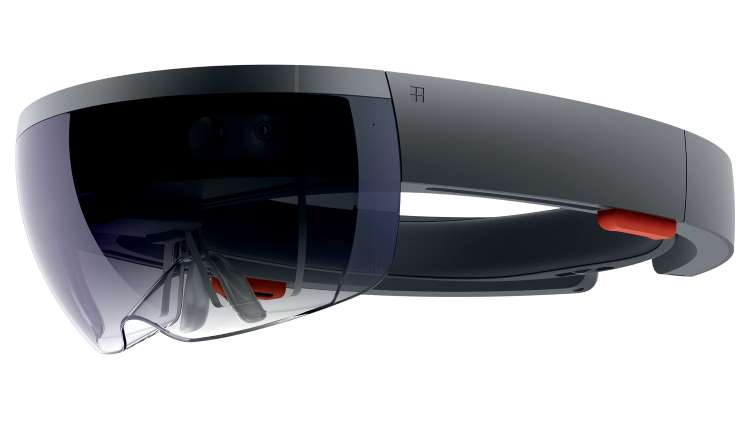
\includegraphics[width=5cm]{Hololens}\label{fig:Hololens}}}%
    \qquad
    \subfloat[Meta 2 \acrshort{acr:AR}-Brille]{{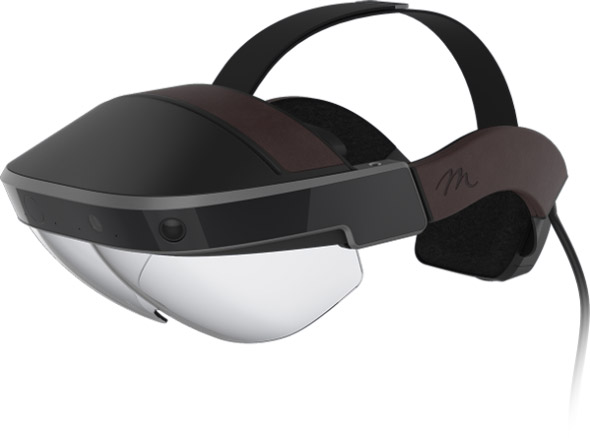
\includegraphics[width=4cm]{Meta2}\label{fig:Meta2}}}%
    \caption{Die zwei potentiellen \acrshort{acr:AR}-Brillen}\label{fig:AR-Brillen}%
\end{figure}

\subsection{\acrshort{acr:VR}-Brillen im Vergleich}
Die, in dieser Arbeit, entwickelte Methode zur \glslink{glos:Labeling}{3D-Datennotation} ist vorwiegend für einen normalen Arbeitsplatz im Büro konzipiert, also einen Platz an dem man einen Desktop-Computer zur Verfügung hat. Deswegen macht es keinen Sinn \acrshort{acr:VR}-Brillen in Betracht zu ziehen die von einem mobilen Gerät betrieben werden (Samsung Gear VR), da diese deutlich weniger Leistung und eine schlechtere Bedienung haben als Geräte für einen Desktop-PC. Auch die Nutzung der Playstation VR ist nicht sinnvoll, da zum Betrieb eine Playstation 4 nötig ist, welche in den wenigsten Unternehmen vorhanden sein dürfte.

Für das \glslink{glos:Labeling}{Klassifizieren} im dreidimensionalen Raum ist eine gute Darstellung und Bedienung notwendig. Bei \acrshort{acr:VR}-Brillen, die einen Desktop-PC als Recheneinheit haben wird beides geboten. Durch die hohe Leistung eines performanten Computers kann der dreidimensionale Raum hochauflösend dargestellt werden. Auch die genaue, für Spiele konzipierte, Steuerung über Controller kommt einem \glslink{glos:Labeling}{Labeling}-Tool zugute. Zum Zeitpunkt der Erstellung dieser Arbeit, gibt es zwei relevante VR-Brillen aus dieser Sparte, die Oculus Rift und die HTC Vive.

\subsubsection{Oculus Rift}
Mit 470 Gramm ist die Oculus Rift (vgl. Abbildung \ref{fig:Oculus}) deutlich leichter als andere Modelle, wie beispielsweise die HTC Vive mit 600 Gramm oder die Playstation VR mit 610 Gramm \cite{bib:OculusTestTragekomfort}. Dies ist für längeres Arbeiten mit ihr sehr vorteilhaft, da schwere Brillen oft schon nach kurzer Zeit störend beim Tragen sind. Des weiteren lässt sich die Brille problemlos an jedem handelsüblichen Büro-Arbeitsplatz verwenden. \textit{\glqq Oculus empfiehlt, die Kameras im Abstand von zwei Metern nebeneinander zu platzieren – bei einem klassischen PC-Arbeitsplatz also links und rechts neben dem Monitor. Das funktioniert in der Praxis gut, man kann sich mit diesem Aufbau ungefähr jeweils einen Schritt in alle Richtungen bewegen\grqq} \cite{bib:OculusTouchTest}. Auch in Sachen Steuerung ist die Oculus Rift anderen Modellen überlegen. Durch die sogenannten Touch Controller, mit denen man virtuell nicht nur Greifen, sondern auch Daumen und Zeigefinger bewegen kann, gelingen ihr \textit{\glqq deutlich feinere Bewegungen\grqq} als beispielsweise der HTC Vive \cite{bib:OculusTouchTest}. Dies bietet für die Entwicklung einer Lösung zur Markierung vieler Objekte zahlreiche Möglichkeiten.\\

Was bei der Oculus Rift nicht so gut funktioniert, wie bei anderen Brillen ist das \gls{glos:Roomscaling}, also das Erfassen der Bewegungen des Benutzers durch einen größeren Raum. Hierfür gibt es bei der Rift zwei Methoden, einmal mit zwei Kameras (kleine Überwachungsfläche) die sich im Abstand von drei Metern in zwei Raumecken gegenüberstehen und eine mit drei Kameras (größere Überwachungsfläche). Beide Methoden funktionieren nicht einwandfrei und auch nicht so gut wie bei der HTC Vive \cite{bib:OculusTouchTest}.

\subsubsection{HTC Vive}
Die HTC Vive (vgl. Abbildung \ref{fig:Vive}) punktet mit dem ausgeklügelten Lighthouse Tracking System, welches in Zusammenarbeit mit VALVE entwickelt wurde \cite{bib:Lighthouse}. Das System kann die Kopfbewegungen des Benutzers durch mehr als 70 Sensoren, welche sowohl in die Brille integriert als auch extra positioniert sind, auf bis zu ein zehntel eines Grades messen \cite{bib:ViveTest}. Auch die Controller werden durch dieses System erfasst, was zu einer genauen Übertragung der physischen Handbewegungen in die virtuelle Welt führt. Dies kommt der Auswahl zahlreicher Objekte, wie es bei der Klassifizierung von Punkten der Fall ist, sehr entgegen. Auch eine gute Darstellung ist dank zweier Displays gewährleistet, die jeweils eine Auflösung von 1080 auf 1200 Pixel haben. Bei diesen Displays kommt es weder zu Verzerrungen des Bildes (\textit{\glqq lens distortion\grqq} \cite{bib:ViveTest}) noch zu Pixelfehlern. Ebenfalls nützlich, vor allem am Arbeitsplatz, ist die Bluetooth-Funktion der Vive. Damit ist es möglich sein Smartphone mit der Brille zu verbinden und somit eingehende Emails oder Ähnliches zu lesen und zu beantworten, ohne die Brille absetzen zu müssen.\\  

Der große Unterschied zwischen Vive und Rift liegt bei der Bedienung durch die unterschiedlichen Controller. Hier hat die HTC-Brille das Nachsehen, weil sie durch Anatomie der Controller weniger Möglichkeiten zur Interaktion in der virtuellen Umgebung bietet. Die sogenannten Wands bieten nämlich keinerlei Funktionen die es ermöglichen eine Hand nachzuahmen, um beispielsweise einzelne Finger zu bewegen und somit virtuelle Objekte greifen zu können. Im Hinblick auf eine durchdachte Steuerung für die Auswahl und Markierung vieler Punkte in einer Punktwolke gibt es somit weniger Möglichkeiten diese zu entwickeln.

\begin{figure}%
    \centering
    \subfloat[HTC Vive \acrshort{acr:AR}-Brille mit Controllern]{{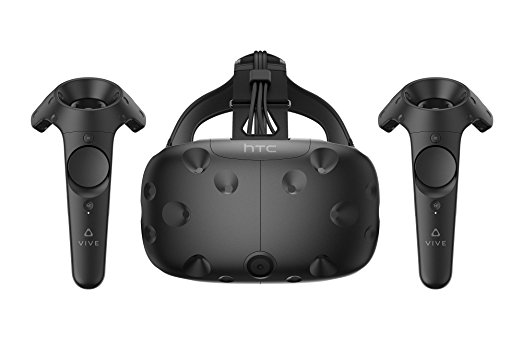
\includegraphics[width=5cm]{Vive}\label{fig:Vive}}}%
    \qquad
    \subfloat[Oculus Rift \acrshort{acr:VR}-Brille mit Controllern]{{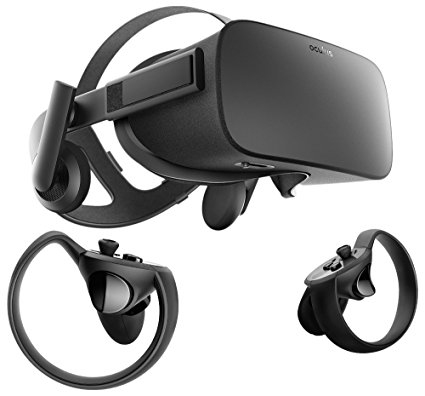
\includegraphics[width=3cm]{Oculus}\label{fig:Oculus}}}%
    \caption{Die zwei potentiellen \acrshort{acr:VR}-Brillen}\label{fig:VR-Brillen}%
\end{figure}

\subsection{Zusammenfassung und Entscheidung}
Für die Wahl des passenden Mediums, auf dem das dreidimensionale \glslink{glos:Labeling}{Labeling} entwickelt werden soll, sind mehrere Faktoren entscheidend. Diese Faktoren ergeben sich danach, wie sehr sich etwas für die genannte Anwendung eignet. Zunächst ist es wichtig eine Punktwolke deutlich und nach Möglichkeit im richtigen Maßstab darzustellen. Hier kommt die \acrlong{acr:AR}-Technologie, durch die Interaktion mit der Umgebung und der lichtempfindlichen Darstellung digitaler Inhalte, sicherlich an ihre Grenzen. In der virtuellen Realität dagegen kann eine solche Wolke problemlos bei jeder Bedingung angezeigt werden, da die reale Umgebung nicht berücksichtigt wird. Sogar der Maßstab kann gut eingehalten werden, da dem virtuellen Raum keine Grenzen gesetzt sind, sodass beliebig große Umfeldmodelle an jedem Arbeitsplatz dargestellt werden können.

Auch die Steuerung spricht für den Einsatz von \acrlong{acr:VR}. Zwar ist das Konzept der Greif-Steuerung der Meta 2 ein guter Ansatz, da diese aber noch nicht zuverlässig und genau funktioniert, ist sie für die Selektion vieler Objekte nicht gut geeignet. Dagegen bietet die Steuerung durch Controller bei \acrshort{acr:VR}-Brillen deutlich mehr Möglichkeiten eine gute Bedienung für das gewünschte Tool zu entwickeln. Die Tasten eines solchen Controllers können vom Entwickler nämlich nach Wunsch programmiert werden wogegen die Gesten für \acrshort{acr:AR}-Brillen nicht verändert bzw. nicht neu erstellt werden sollten \cite{bib:NewGesture}. 

Zudem gibt es, durch die deutlich frühere Markteinführung, viel mehr Dokumentationen und Hilfestellungen im Bereich \acrlong{acr:VR}, was die Entwicklung deutlich erleichtert.

Aufgrund der eben genannten Vorteile von \acrshort{acr:VR} gegenüber \acrshort{acr:AR} wird für die Entwicklung, im Rahmen dieser Arbeit, \textbf{\acrlong{acr:VR}} verwendet.\\

Bleibt noch die Frage zu klären welche Brille verwendet werden soll. Diese Frage ist schwerer zu beantworten als die vorherige. Die zwei potentiellen \acrshort{acr:VR}-Brillen, also Oculus Rift und HTC Vive, sind beide geeignete Kandidaten. Die Vive punktet durch gutes \gls{glos:Roomscaling} und gutes Tracking der Brille und der Controller, wogegen die Oculus Rift guten Tragekomfort und gut durchdachte Controller-Bedienung bietet. 

Wichtig für die Entwicklung einer \glslink{glos:Labeling}{3D-Datennotation} ist aber nicht, ob man sich physisch, also mittels \gls{glos:Roomscaling} durch die Punktwolke bewegen kann, sondern wie man die klassifizierbaren Punkte markieren bzw. auswählen kann. Da hierfür die Oculus Touch Controller mehr Möglichkeiten bieten wird für die Entwicklung eines \acrshort{acr:VR}-\glslink{glos:Labeling}{Labeling}-Tools die \textbf{Oculus Rift} verwendet.    

\section{Wahl des passenden Rechners}
Für die Berechnungen, die notwendig sind um Inhalte in der Oculus anzuzeigen, ist nicht die Brille selbst verantwortlich. Diese Aufgabe übernimmt ein extra Computer. Die Brille fungiert dementsprechend nur als Anzeigegerät. Auch die Sensoren sind an den PC angeschlossen um das Tracking der Brille und der Controller zu gewährleisten. Da vor allem die Grafikberechnungen sehr aufwendig sind, kann nicht jeder handelsübliche PC oder Laptop dazu verwendet werden eine solche \acrshort{acr:VR}-Brille zu betreiben.\\ 

Wichtig sind also zunächst die Basiskomponenten wie ein schneller Prozessor und eine leistungsstarke Grafikkarte. Aber auch ein schneller Arbeitsspeicher mit ausreichender Kapazität ist wichtig damit notwendige Daten so schnell wie möglich zur Verfügung stehen. Für die Wahl, welche Komponenten eingesetzt werden sollen, kann sich an den empfohlenen Spezifikationen des Herstellers orientiert werden (Oculus Rift Recommended System Specs \cite{bib:OculusSpecs}). Diese sind jedoch vorwiegend für den Endnutzer gedacht, bei dem es wichtig ist ein einzelnes Programm für die Brille auszuführen. Für die Entwicklung ist dagegen mehr Leistung notwendig. Soll zum Beispiel eine erstellte Software getestet werden, muss nicht nur die Software selber, sondern eventuell auch die Entwicklungsumgebung und zusätzliche \glslink{glos:Debugger}{Debugging-} und  Analyse-Tools ausgeführt werden. An dieser Stelle sollte also nicht gespart werden.\\

Sind die Basiskomponenten ausgewählt, sollte noch geprüft werden ob noch weiteres Zubehör wichtig ist um diese zu betreiben. Da gerade Prozessoren mit hoher \gls{glos:Taktrate} viel Wärme produzieren, muss stets für ausreichende Kühlung gesorgt werden. Bei der Rechner-Konfiguration für diese Masterarbeit wurden beispielsweise, neben einem hochwertigen Prozessorkühler, noch zwei weitere Gehäuselüfter verbaut, um die Abwärme aus dem inneren des Computers heraus zu leiten. Zu guter Letzt ist es wichtig ein passendes Mainboard auszuwählen, auf dem alle Komponenten verbaut werden. Für die Oculus Rift werden vier USB-Anschlüsse empfohlen, welche das Mainboard haben muss \cite{bib:OculusSpecs}. Ebenfalls muss das Board genug Platz bieten um die gewählten Komponenten zusammen anbringen zu können. Leistungsstarke Grafikkarten und Prozessorlüfter können zum Teil sehr groß ausfallen. Auch für weitere Aufrüstungen sollte das Board genügend Platz bieten, falls es, zu einem späteren Zeitpunkt, notwendig wäre zusätzliche Komponenten (zweite Grafikkarte) hinzuzufügen. Unter Berücksichtigung der eben genannten Aspekte wurde folgende Rechner-Konfiguration für die Entwicklung verwendet:\\  

\begin{table}[h]
 \begin{tabular}{lcr}
  \textbf{Bezeichnung der Komponente} & \textbf{Verwendete Komponente}\\
  \\
  
  \textit{Prozessor:} & Intel® Core™ i7-7700K\\
  \textit{Grafikkarte:} & Gainward GeForce GTX 1070 Phoenix\\
  \textit{Mainboard:} & ASUS PRIME Z270-A\\
  \textit{Arbeitsspeicher(RAM):} & HyperX DIMM 16 GB DDR4-2400 Kit\\
  \textit{Festplatte:} & Samsung 850 Pro 2,5"\ 512 GB\\
  \textit{Netzteil:} & Cooler Master G550M 550W\\
  \textit{Prozessorlüfter:} & Noctua NH-D9L\\
  \textit{Gehäuselüfter:} & 2x Coolink SWiF2-1200 120x120x25\\
  \textit{Gehäuse:} & Cooler Master N300\\
\\
 \end{tabular}
 \caption{Rechner-Konfiguration für die Entwicklungen dieser Arbeit}
 \label{tab:Rechnerkonfig}
 \end{table}

\section{Wahl der passenden Entwicklungsplattform}
Für die Erstellung von \acrlong{acr:VR} Software gibt es zwei Entwicklungsumgebungen, die gut für das Entwickeln von \acrlong{acr:VR} geeignet sind, weil sie schon seit längerem \acrshort{acr:VR}-Support bieten und dies auf umfassende Weise. Diese sind  Unreal Engine 4 und Unity Engine. Beide Plattformen bieten alles nötige um \acrshort{acr:VR}-Software zu entwickeln, weshalb die Wahl zwischen ihnen eher subjektiv, aufgrund der eigenen Bedürfnisse und Erfahrungen, zu fällen ist. 

Im Allgemeinen kann man sagen, dass die Unreal Engine mehr Möglichkeiten für professionelles Game Engineering bietet, da viel Wert auf visuelle Qualität gelegt wird, beispielsweise durch integrierte \gls{glos:PostPr}-Techniken und bessere \gls{glos:Shader}. Sie bietet neben dem \gls{glos:Scripting} auch die Gelegenheit, durch C++ Programmierung Module der Engine zu verändern bzw. neue hinzuzufügen. Das gestalten von \glspl{glos:UI} ist mit dem UMG UI Designer ebenfalls gut gelöst \cite{bib:UEvsUE4}.

Die Unity Engine bietet vor allem Anfängern einen leichten Einstieg in die Welt der Grafik- und Spieleprogrammierung. Im Editor können ganz einfach sogenannte Game Objects erstellt werden, denen dann Funktionalitäten und Eigenschaften angehängt werden können. Dies geschieht meist in Form von Skripten, welche oft schon vorgefertigt zur Verfügung stehen. Wenn dies nicht der Fall ist können diese angepasst oder neu erstellt werden. Die große Community der Unity Engine ist hierbei eine große Hilfe.

\subsubsection{Entscheidung}
Ein Vorteil den die Unity Engine, im Falle dieser Arbeit, bietet ist Nutzung von C\# als \gls{glos:Scripting}-Sprache. Da  
C.LABEL (vgl. \ref{sec:C.LABEL}) ebenfalls in C\# programmiert wurde können Komponenten, wie etwa das Einlesen von Daten in die Anwendung, leicht übernommen werden. Des Weiteren habe ich selbst schon, im Rahmen eines Universitätsprojekts, mit dieser Engine gearbeitet, weshalb ein längeres einarbeiten in die Entwicklungsumgebung nicht nötig wäre. Die Vorteile der Unreal Engine sind, wie schon erwähnt, die visuelle Präsentation und die dabei gebotene Performance. Diese sind vor allem für das erstellen aufwändiger Landschaften und deren Inhalten von Vorteil. 

Für die Entwicklung der, in dieser Arbeit, angestrebten Anwendung spielen jedoch Dinge wie Grafik und beeindruckendes Leveldesign keine große Rolle. Viel wichtiger ist sowohl die Möglichkeit der Kompatibilität zur C.LABEL-Anwendung als auch die vorhandene Entwicklungserfahrung einer Engine. Gerade letzteres ist auf Grund des begrenzten Zeitrahmens einer Masterarbeit von Vorteil, da ohne große Einarbeitung mehr Zeit zum Entwickeln von Funktionalität und Optimierungen bleibt. Aus diesen Gründen wird im weiteren Verlauf dieser Arbeit die \textbf{Unity Engine} als Entwicklungsumgebung verwendet.














%\chapter{Ab hier kommen Inhalte für CopyPaste}
%\chapter{Sections and Paragraphs}

\section{Section}
Inhalt des ersten Abschnitts
\subsection{Subsection}
\label{lab1}
Inhalt des ersten Unterabschnitts
\paragraph{Paragraph!?}
\subparagraph{Unterparagraph!?}

\section{Referenz}
Wie in \ref{lab1} geschrieben.

\chapter{Lists}

\begin{enumerate}
\item erstens
\item zweitens
\begin{itemize}
\item unter erstens
\item unter zweitens
\item[+] Pro
\item[-] Contra
\end{itemize}
\item drittens\\
Das Zeichen \verb|\\| \\ forciert eine neue Zeile.
\end{enumerate}


\chapter{Tabellen}
\begin{tabular}{|l|l|}
left alligned & left alligned----------\\
left alligned------- & left alligned\\
\end{tabular}

\begin{tabular}{|r|r|}
------right alligned & right alligned\\
right alligned & --------right alligned\\
\end{tabular}

\begin{tabular}{|c|c|}
center alligned & center alligned\\
center alligned & center alligned\\
\end{tabular}

\begin{tabular}{|l|r|c|}
left alligned & right alligned & center alligned\\
\end{tabular}

\chapter{Figures}

\begin{figure}[h] %h=here	t=top	b=bottom	p=seperate page 
\centering	%if not centered then left aligned

\includegraphics[width=1\textwidth]{Main_Images/cmoreLogo}
\caption{Here is my image}
\label{image-myimage}
\end{figure}

\chapter{Equations}

$1+2=3$ \\
$$1+2=3$$
\begin{equation}
1+2=3
\end{equation}
\\
\begin{eqnarray}
x_1^2 & = & 1+2+3 \\
& = & \sqrt{6}
\end{eqnarray}


\chapter{References}
This is a reference.\cite{Testzitat}

This is a website reference.\cite{TestWebsite}
%\chapter{Ab hier enden Inhalte für CopyPaste}


\appendix
\chapter{Appendix Title}
%\input{chapters/appendix}



\bibliographystyle{IEEEtran}
\bibliography{Masterarbeit}

\end{document}